In this chapter, we will present the architecture our research proposes in order to evaluate the large-scale re-hosting of router firmware images and the innovative aspects of the approach intended in this project.

\section{Complete Architecture}
This paper represents only part of a solution idealized for a bigger research project, to be conducted throughout the years by a team of researchers. Figure \ref{fig:architecture} illustrates the overview of the architecture for the complete project, whereas in this paper we will only focus on the re-hosting part of the proposed architecture.

\begin{figure}[h]
    \centering
    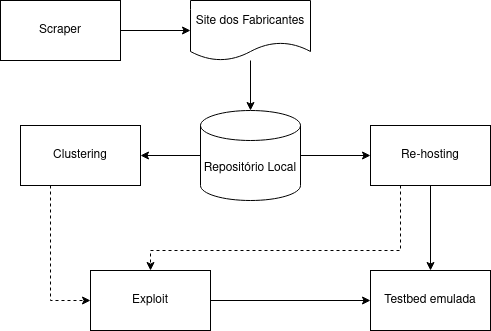
\includegraphics[width=0.65\textwidth]{figs/RehostingDiagram.png}
    \caption{Architecture proposed for a complete solution in firmware vulnerability analysis.}
    \label{fig:architecture}
\end{figure}

The complete architecture includes a scraper module consisting of a web crawler responsible for entering router vendors websites and downloading for a local repository the biggest amount of firmware images available as possible. Firmware images are going to be a requirement for the re-hosting experiments to be conducted. In this stage, the scraper module is going to only serve the purpose of providing a minimum amount of firmware images to allow the research in the re-hosting process. Therefore, our approach will be to use Firmadyne's \cite{firmadyne} implemented scraper for now. In the future, if needed, our team is willing to update Firmadyne's \cite{firmadyne} scraper and also add more vendors to the list.

From the local repository, two different modules will perform actions using the acquired firmware. The re-hosting module will be responsible for extracting firmware images (and collecting information about the firmware in the process) and preparing the firmware image to be emulated. As this module will be the focus of this research, section \ref{sec:re-hosting} will explain this process in detail. The other module to perform actions in firmware images contained in the local repository is the clustering module. This consists on searching for similarities and patterns amongst different firmware images. The results obtained by the clustering modules can be used in further steps to improve the vulnerability analysis and discovery process.

The final module of the architecture is the exploitation module. In this stage, vulnerability analysis (using frameworks to detect known software vulnerabilities) and vulnerability discovery (such as fuzzing techniques) will be applied on the emulated firmware to analyze its security performance.

\section{Firmware Extraction}
\label{sec:extraction}

For the firmware extraction process, our research is going to focus on enhancing the original script provided with Firmadyne \cite{firmadyne} for firmware extraction developed in Python and making extensive use of {\tt binwalk}'s API. This original script uses {\tt binwalk} to recursively extract the firmware image setting a limit for depth and breadth in order to limit this process as it is very slow. To speed up the extraction, the {\tt /tmp} directory of the host system (which is used to temporarily store files during the firmware extraction process) is going to be mounted on the {\tt tmpfs} provided by the Linux kernel and that allow us to mount a directory in the RAM instead of mounting it on the disk.

Some firmware images can't be automatically extracted using this method. After executing the script in all firmware images, we will then check which were not successfully extracted in the automated process. Some of these will be manually extracted in order to identify if and how the extraction process could be modified to be able to also extract this image. After modifying the extraction script, this entire process will be repeated until our team is satisfied with the amount of extracted firmware images.

\section{Re-hosting Process}
\label{sec:re-hosting}

During the re-hosting phase, our objective is to be able to run software intended to run in the original firmware without really having the original hardware in which it was designed to run. Firmadyne's \cite{firmadyne} approach to firmware re-hosting is to extract from the original firmware image its original root filesystem and kernel. It then completely ignores the original kernel, and replace it with a custom instrumented kernel designed by the researchers (they developed one instrumented kernel for {\tt ARM} architecture and one for {\tt MIPS} architecture). Finally, the emulation process is done by the {\tt QEMU} tool, that uses binary translation to allow execution of binaries from different architectures. The emulated firmware is emulated with {\tt QEMU} using the instrumented kernel together with the extracted filesystem from the original firmware.

Our approach to firmware re-hosting will be similar to Firmadyne's \cite{firmadyne} approach, with differences in regard to the kernel replacement part. Instead of just building one heavily instrumented kernel and replacing all firmware images with that same instrumented kernel, we propose building specific kernel versions on demand according to the original kernel used by the firmware image being emulated. With that, our hope is that using a kernel more similar with the original one could reduce incompatibility with network drivers and modules and therefore increase the number of emulated firmware with a working network interface, allowing us to extend the vulnerability analysis and discovery process to a bigger amount of router firmware images than the one covered by the original Firmadyne's \cite{firmadyne} implementation.

This process of automated kernel cross-compilation, however, faces a lot of issues. The first one is how to define a valid kernel compile configuration that results in a kernel that has the features expected in a router firmware. Kernel compile configuration is a configuration file ({\tt .config}) where the user can configure a large list of parameters regarding the kernel that will be compiled.

These configuration files can be filled up by the user manually or via answering questions interactively in the command line interface, or it can also be extracted from an already existing compiled kernel in execution. Defining how to produce an adequate {\tt .config} file is already an open problem in our research. Other idea is to extract kernel compilation default configuration from OpenWrt Linux systems. The OpenWrt is a Linux developed to be used as an open-firmware for wireless routers. That being said, it is possible that OpenWrt images have kernel configurations that are compatible with most networking features expected from a wireless router. In this way, in this research, we plan to investigate the better way to produce a valid compilation configuration file in order to allow kernel compiling.

After choosing a valid kernel compilation configuration file, the kernel has to be cross-compiled in the host machine, so that it is compiled for the architecture expected in the original firmware image. Kernel cross-compilation is also a very difficult task, as the compilation process is heavily dependent on its toolchain (compiler, utilities and libraries versions). This means that in order to automatically compile multiple different kernel versions, there has to be a way to automatically switch between a set of known working toolchains for each kernel version.

Finally, after compiling a kernel version that matches the original kernel, the firmware image is then ready to be emulated using the {\tt QEMU}. Firmware will be emulated using the newly compiled kernel with the original filesystem extracted from the firmware sample. After that, following the work of \cite{firmadyne}, we will evaluate if these emulated firmware images can infer and configure the network successfully. If that is the case, then vulnerability analysis and discovery techniques will be applied (using common tools for this purpose). The results obtained will be used to evaluate overall firmware security and the mapped vulnerable products (if that happens) will be reported back to the vendor.